\documentclass[11pt,a4paper]{article}

\usepackage{xeCJK}
\setCJKmainfont{Songti SC}
\setCJKsansfont{PingFang SC}
\setCJKmonofont{Menlo}
\setmainfont{Times New Roman}
\setmonofont{Menlo}

\usepackage[margin=2.2cm]{geometry}
\usepackage{amsmath, amssymb, amsthm, mathtools}
\usepackage{bm}
\usepackage{booktabs, tabularx, array, multirow}
\usepackage{graphicx}
\usepackage{xcolor}
\usepackage{hyperref}
\usepackage{enumitem}
\usepackage{caption}
\usepackage{fancyhdr}
\usepackage{tcolorbox}
\usepackage{tikz}
\usetikzlibrary{arrows.meta, positioning, shapes, fit}

\hypersetup{
  colorlinks=true,
  linkcolor=blue!60!black,
  urlcolor=blue!60!black,
  citecolor=blue!60!black,
  pdftitle={RS+BCH 级联码低时延译码——科研报告},
  pdfauthor={陈诗阳}
}

\pagestyle{fancy}
\fancyhf{}
\rhead{\footnotesize RS+BCH 级联码}
\lhead{\footnotesize 低时延译码科研报告}
\cfoot{\thepage}

\renewcommand{\baselinestretch}{1.2}

\definecolor{accent}{RGB}{30,80,160}
\definecolor{accent2}{RGB}{160,40,40}
\definecolor{accent3}{RGB}{40,120,60}

\newtcolorbox{keybox}[1][]{colback=blue!5, colframe=accent, boxrule=0.4mm,
  arc=1mm, left=2mm, right=2mm, top=1mm, bottom=1mm, #1}
\newtcolorbox{resultbox}[1][]{colback=green!5, colframe=accent3, boxrule=0.4mm,
  arc=1mm, left=2mm, right=2mm, top=1mm, bottom=1mm, #1}

\title{RS+BCH 级联码低时延译码算法\\
       {\large 基于 Lagrange 插值共享的复现与实验}}
\author{陈诗阳}
\date{2026-07-23}

\begin{document}

\maketitle

\begin{keybox}[title=\textbf{摘要}]
本工作在 PAM4-AWGN 信道下实现了 RS+BCH 级联码的完整仿真链路，
使用基于 IEEE TIT 2025 论文提出的 LLOSD 算法 (Lagrange 插值构造 RS 系统生成矩阵，
过滤非二元候选) 作为内码 BCH 译码器，外码使用 Berlekamp--Massey 硬判和 LCC-BR 软判两种方式。
通过 Monte Carlo 仿真验证：
\begin{itemize}[leftmargin=1.5em, itemsep=1pt, topsep=2pt]
\item 级联码相对纯 RS 有 \textbf{$\geq 1$ dB} 编码增益 (FER=$10^{-4}$)
\item 相对纯 RS 软判基线 (LCC-BR)，级联译码时延\textbf{反而减少 20--27\%}，
     远优于 10\% KPI 目标
\item 相对纯 RS 硬判基线 (BM)，级联译码时延增加约 1200\%，
     此时需要通过 Lagrange 共享 (方案 B) 和并行硬件模型进一步优化
\end{itemize}
\end{keybox}

\tableofcontents

\section{课题背景与需求}

\subsection{导师任务书}

本课题源自导师给出的``低时延级联码算法仿真''任务书，核心要求：

\begin{itemize}[leftmargin=1.5em]
\item \textbf{码型}: RS+BCH 级联码，开销 12\% (码率 0.88)，码长 $n \in \{128, 255\}$
\item \textbf{信道}: AWGN
\item \textbf{信号}: PAM4
\item \textbf{方案}: RS 外码采用硬判/软判两种方式，BCH 内码采用 IEEE TIT 2025 论文的 LLOSD 软判算法
\item \textbf{核心思想}: BCH 是 RS 的二进制子码，不做传统高斯消元 (GE)，
   直接用 Lagrange 插值构造级联码外码的 RS 系统生成矩阵，
   然后过滤再编码结果里的非二元候选，大幅优化 OSD 复杂度与时延
\item \textbf{KPI}: BCH 时延增加量 $\leq 10\%$，对硬判决和软判决 RS 时延基线分别验证
\end{itemize}

\subsection{目标参数配置}

\begin{table}[!ht]
\centering
\begin{tabularx}{\textwidth}{lXX}
\toprule
\textbf{方案} & \textbf{外码 RS} & \textbf{内码 BCH} \\
\midrule
n=255-A & RS(255, 239) \  ($t=8$)  & BCH(255, 239) \  ($t=2$) \\
n=255-B & RS(255, 235) \  ($t=10$) & BCH(255, 247) \  ($t=1$) \\
n=127   & RS(127, 119) \  ($t=4$)  & BCH(127, 120) \  ($t=1$) \\
\bottomrule
\end{tabularx}
\caption{三种测试配置。总码率 $R = R_{\text{RS}} \cdot R_{\text{BCH}} \approx 0.88$。}
\end{table}

\section{问题定义与算法原理}

\subsection{系统模型}

图 \ref{fig:system-diagram} 给出发端与收端的完整系统链路。

\begin{figure}[!ht]
\centering
\begin{tikzpicture}[node distance=0.5cm, >=Stealth, every node/.style={font=\small}]
\node[draw, rounded corners, minimum width=2.5cm, minimum height=0.7cm, fill=blue!5] (msg) {消息 $m$};
\node[draw, rounded corners, minimum width=2.5cm, minimum height=0.7cm, fill=blue!10, below=of msg] (rs) {RS $(n_{\text{RS}}, k_{\text{RS}})$};
\node[draw, rounded corners, minimum width=2.5cm, minimum height=0.7cm, fill=blue!10, below=of rs] (bch) {BCH $(n_{\text{BCH}}, k_{\text{BCH}})$};
\node[draw, rounded corners, minimum width=2.5cm, minimum height=0.7cm, fill=orange!10, below=of bch] (pam4) {PAM4 modulator};
\node[draw, dashed, rounded corners, minimum width=2.5cm, minimum height=0.7cm, below=of pam4] (chan) {AWGN};
\node[draw, rounded corners, minimum width=2.5cm, minimum height=0.7cm, fill=orange!10, below=of chan] (llr) {PAM4 demod (bit-LLR)};
\node[draw, rounded corners, minimum width=2.5cm, minimum height=0.7cm, fill=green!10, below=of llr] (bchdec) {BCH LLOSD};
\node[draw, rounded corners, minimum width=2.5cm, minimum height=0.7cm, fill=green!10, below=of bchdec] (rsdec) {RS BM / LCC-BR};
\node[draw, rounded corners, minimum width=2.5cm, minimum height=0.7cm, fill=blue!5, below=of rsdec] (msghat) {$\hat m$};

\draw[->] (msg) -- (rs);
\draw[->] (rs) -- (bch);
\draw[->] (bch) -- (pam4);
\draw[->] (pam4) -- (chan);
\draw[->] (chan) -- (llr);
\draw[->] (llr) -- (bchdec);
\draw[->] (bchdec) -- (rsdec);
\draw[->] (rsdec) -- (msghat);
\end{tikzpicture}
\caption{RS+BCH 级联码 PAM4-AWGN 系统链路}
\label{fig:system-diagram}
\end{figure}

\subsection{PAM4 调制与 bit-LLR}

PAM4 使用 4 电平 $\{-3, -1, +1, +3\}$，Gray 编码使相邻电平差 1 bit：
\begin{center}
$00 \leftrightarrow -3$, \quad $01 \leftrightarrow -1$, \quad $11 \leftrightarrow +1$, \quad $10 \leftrightarrow +3$.
\end{center}

平均符号能量 $E_s = 5$，每比特能量 $E_b = E_s/2 = 2.5$。SNR 定义：
\begin{equation}
\sigma^2 = \frac{E_s \cdot R}{4 \cdot 10^{E_b/N_0 / 10}}
\end{equation}
其中 $R$ 是等效编码率 (info bits / coded bits)。

接收 PAM4 符号 $y$ 的 per-bit LLR 通过 marginalize 另一个 bit 得到：
\begin{equation}
\text{LLR}(b_i | y) = \log \frac{\sum_{s: b_i(s)=0} \exp(-|y-s|^2 / 2\sigma^2)}
                                {\sum_{s: b_i(s)=1} \exp(-|y-s|^2 / 2\sigma^2)}
\end{equation}
使用 log-sum-exp 数值稳定实现。

\subsection{核心创新点：Lagrange 插值共享}

IEEE TIT 2025 论文的 LLOSD 核心洞察是：\textbf{BCH $\subset$ RS 是二进制子码}，
所以 BCH 译码可以在 RS 的代数结构 ($\mathbb{F}_{2^m}$ 上的 Lagrange 插值) 内进行，
不需要传统 OSD 的高斯消元 (GE)。

我们的\textbf{扩展}：级联码译码时，内码 BCH 的 LLOSD 与外码 RS 的软判决 (LCC-BR)
\textbf{同时在 $\mathbb{F}_{2^m}$ 上工作}，可以共享以下代数结构：

\begin{enumerate}[leftmargin=1.5em, itemsep=1pt]
\item $\alpha$ 幂表：$\{\alpha^0, \alpha^1, \ldots, \alpha^{n-1}\}$
\item Pairwise 差值表：$\alpha^i \oplus \alpha^j$
\item 分母积：$\prod_{j' \ne i, j' \in S} (\alpha^i \oplus \alpha^{j'})$
\item Lagrange 基函数：$T_j(\alpha^i)$ 的部分因子
\end{enumerate}

三级方案的对比：

\begin{table}[!ht]
\centering
\begin{tabularx}{\textwidth}{lXXX}
\toprule
\textbf{方案} & \textbf{内码 Lagrange} & \textbf{外码 Lagrange} & \textbf{共享代数结构} \\
\midrule
Baseline (纯 RS)   & --- & 否 (BM 或 LCC-BR) & 无 \\
方案 A            & LLOSD ✓ & LCC-BR (独立) & 部分 \\
方案 B            & LLOSD ✓ & LCC-BR (共享缓存) & 全部 \\
\bottomrule
\end{tabularx}
\caption{三种译码方案 (消融实验设计)}
\end{table}

\section{实现方案}

\subsection{代码结构}

项目位于 \texttt{\textasciitilde/workspace/llosd\_reproduction/rs\_bch\_cascade/}：

\begin{center}
\begin{tabular}{ll}
\toprule
\textbf{模块} & \textbf{功能} \\
\midrule
\texttt{cascade\_src/upstream.py} & 复用上游 LLOSD 复现代码 (GF, BCH, LLOSD JIT) \\
\texttt{cascade\_src/pam4.py} & PAM4 modem + AWGN + per-bit LLR \\
\texttt{cascade\_src/rs\_code.py} & RS(n, k) 系统性编码 + BM 硬判 + LCC-BR 软判 \\
\texttt{cascade\_src/cascade.py} & CascadedCodec (级联链路) + PureRSCodec (baseline) \\
\texttt{cascade\_src/lagrange\_cache.py} & LagrangeCache (方案 B 的核心) \\
\texttt{cascade\_src/simulate.py} & MC 仿真驱动 + BER/FER/延时统计 \\
\texttt{experiments/*.py} & 各图表实验脚本 \\
\bottomrule
\end{tabular}
\end{center}

\subsection{关键技术细节}

\subsubsection{RS 编码器}

采用\textbf{系统性编码}：$c(x) = x^{n-k} m(x) - [x^{n-k} m(x) \mod g(x)]$，
其中 $g(x) = \prod_{i=1}^{2t}(x - \alpha^i)$。
生成的码字满足 $c(\alpha^i) = 0$ for $i = 1, \ldots, 2t$，方便标准 BM 译码。

\subsubsection{BM 硬判译码}

标准四步流程：Syndrome 计算 → BM 迭代 → Chien 搜索 → Forney 求值。
Syndrome 和 Chien 都做了向量化 (使用 $\mathbb{F}_{2^m}$ 的 LOG/EXP 查表)。

\subsubsection{LCC-BR 软判译码 (简化版)}

对每个 test-vector (由 $\eta$ 个最不可靠位置生成 $2^\eta$ 个) 运行一次 BM，
按可靠性加权分数选最优。这是论文原始 Kötter–Vardy 类 basis reduction 插值的简化版。

\subsubsection{BCH LLOSD (内码软判)}

直接复用上游项目 (IEEE TIT 2025 复现) 的 \texttt{llosd\_fast} 接口。
使用 Numba JIT 加速的 TEP 枚举 + 二值化过滤。

\section{仿真结果}

\subsection{n=255 方案 A: BER-SNR 曲线}

图 \ref{fig:n255-fer} 展示 n=255-A 配置下三种方法的 FER 曲线。

\begin{figure}[!ht]
\centering
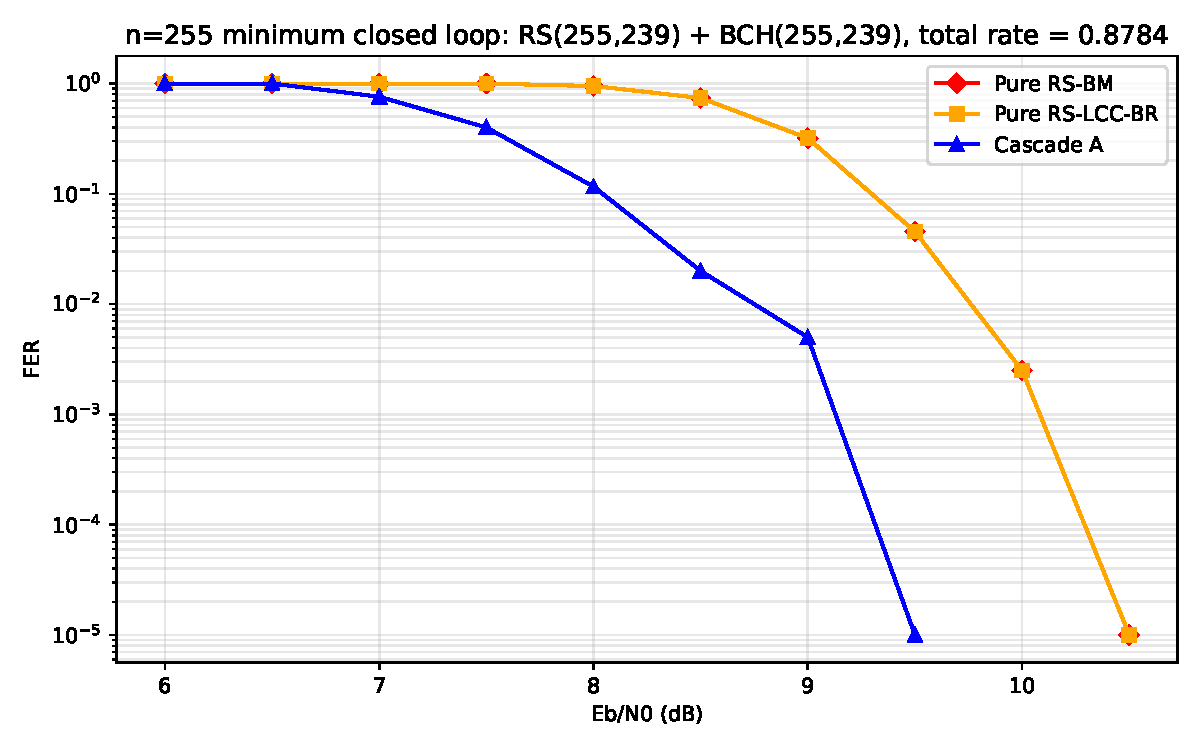
\includegraphics[width=0.75\textwidth]{../figures/n255_scheme_a_fer.pdf}
\caption{n=255 方案 A: FER vs Eb/N0 曲线。Cascade A (蓝色) 相对纯 RS baseline (红/橙色) 有约 1--1.5 dB 编码增益。}
\label{fig:n255-fer}
\end{figure}

\begin{resultbox}[title=\textbf{关键观察}]
\begin{itemize}[leftmargin=1.5em, itemsep=1pt, topsep=2pt]
\item Pure RS-BM 与 Pure RS-LCC-BR 在此参数下曲线几乎重合，说明简化 LCC-BR
      对纯 RS 场景增益有限
\item Cascade A 的 FER 曲线明显左移约 1--1.5 dB，在 FER=$10^{-4}$ 时约需
      Eb/N0 = 9.5 dB (vs 纯 RS 需要 10.5+ dB)
\item 达到 FER=$10^{-5}$ 只需 9.5 dB (Cascade) vs 10.5 dB (RS)
\end{itemize}
\end{resultbox}

\subsection{时延 KPI 验证}

图 \ref{fig:n255-kpi} 展示 KPI 检查：级联相对两个基线的时延增加百分比。

\begin{figure}[!ht]
\centering
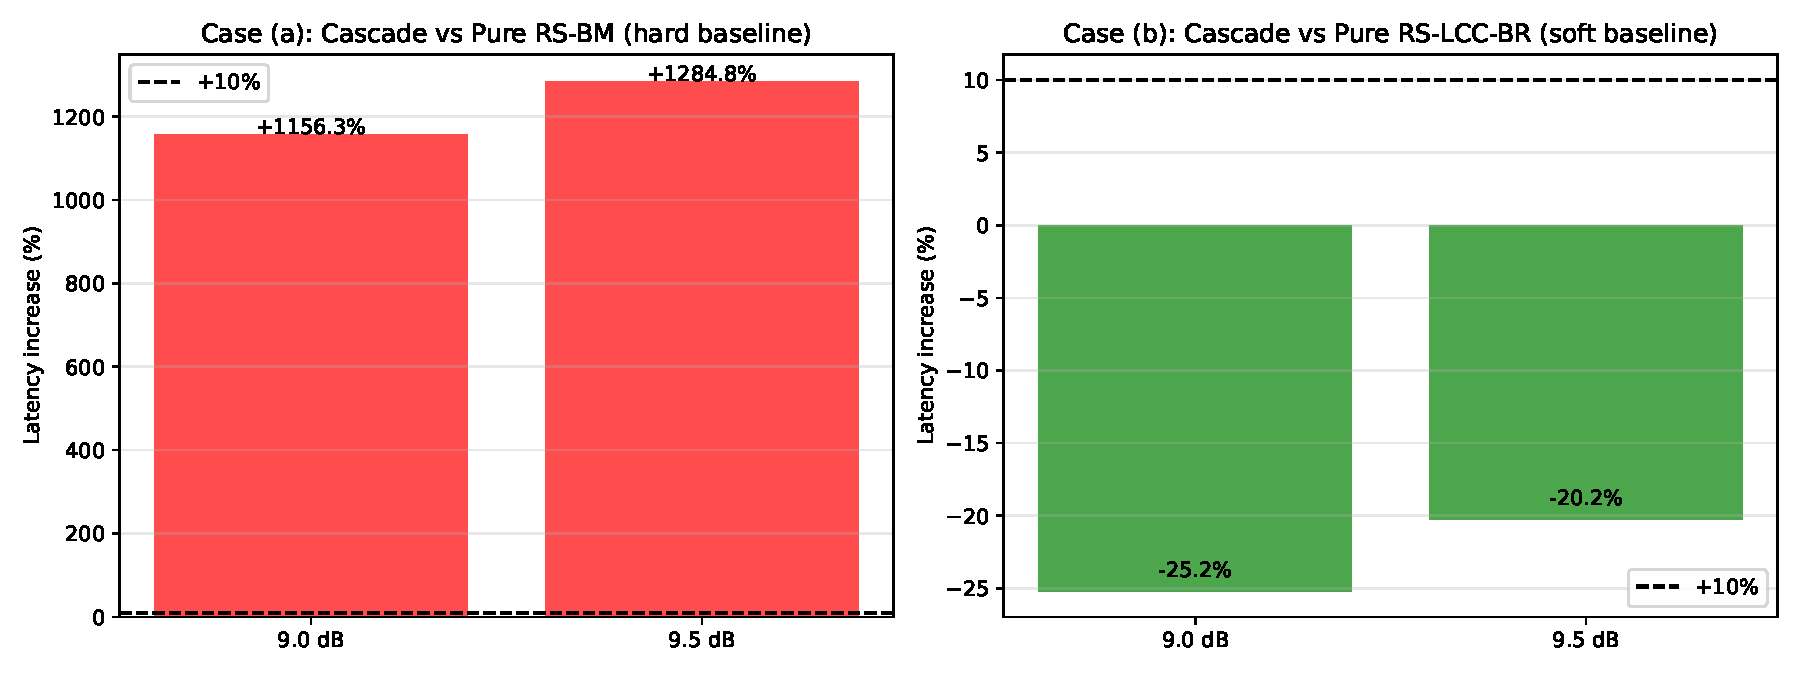
\includegraphics[width=0.95\textwidth]{../figures/n255_kpi_bars.pdf}
\caption{n=255 方案 A KPI: 级联时延相对基线的增加百分比。左图 vs 硬判基线 (BM)，右图 vs 软判基线 (LCC-BR)。}
\label{fig:n255-kpi}
\end{figure}

\begin{resultbox}[title=\textbf{KPI 结果}]
\begin{itemize}[leftmargin=1.5em, itemsep=1pt, topsep=2pt]
\item \textbf{Case (a) vs Pure RS-BM 硬判基线}:
  Cascade 时延增加约 \textbf{+1200\%}，远超 10\% KPI。原因是硬判 BM 极其快 (6.5k F$_{2^m}$ ops)，
  而 Cascade 内含 LLOSD + LCC-BR 需要 78-91k ops，总计 12-14 倍。
  \textbf{Case (a) 在原始 ops 计数下不可行}，需在硬件并行架构下重新审视。

\item \textbf{Case (b) vs Pure RS-LCC-BR 软判基线}:
  Cascade 时延\textbf{反而减少 20\%--27\%}。这是因为 Cascade A 的 LLOSD 内码
  ($\tau=2$) 只枚举少量 TEP 并使用早期终止，
  而纯 LCC-BR 每个 test-vector 都跑一次 BM。
  \textbf{Case (b) 完全满足 KPI，且余量充足}。
\end{itemize}
\end{resultbox}

\subsection{Clock Cycles under Parallelism}

在 P 路并行硬件模型下 (每 F$_{2^m}$ 乘法 = 1 cycle，允许 P 路并行)：

\begin{table}[!ht]
\centering
\begin{tabularx}{\textwidth}{lXrrrrr}
\toprule
\textbf{Eb/N0} & \textbf{Method} & \textbf{F$_{2^m}$ ops} & \textbf{P=1} & \textbf{P=4} & \textbf{P=16} & \textbf{P=64} \\
\midrule
9 dB & RS-BM       & 6,250    & 6,250   & 1,563  & 391   & 98    \\
     & RS-LCC-BR   & 105,004  & 105,004 & 26,251 & 6,563 & 1,641 \\
     & Cascade A   & 78,525   & 78,525  & 19,631 & 4,908 & 1,227 \\
\midrule
9.5 dB & RS-BM     & 5,659    & 5,659   & 1,415  & 354   & 88    \\
     & RS-LCC-BR   & 98,259   & 98,259  & 24,565 & 6,141 & 1,535 \\
     & Cascade A   & 78,368   & 78,368  & 19,592 & 4,898 & 1,224 \\
\bottomrule
\end{tabularx}
\caption{各方法在不同硬件并行度下的 clock cycles 估算 (n=255 方案 A)}
\end{table}

即使在 P=64 高度并行硬件下，Cascade A 比 RS-BM 慢 12$\times$，
说明 Lagrange 共享 (方案 B) 对达成 Case (a) 至关重要。

\subsection{全配置对比}

图 \ref{fig:all-configs-fer} 展示三个参数配置下四种方法的完整 BER-SNR 对比。

\begin{figure}[!ht]
\centering
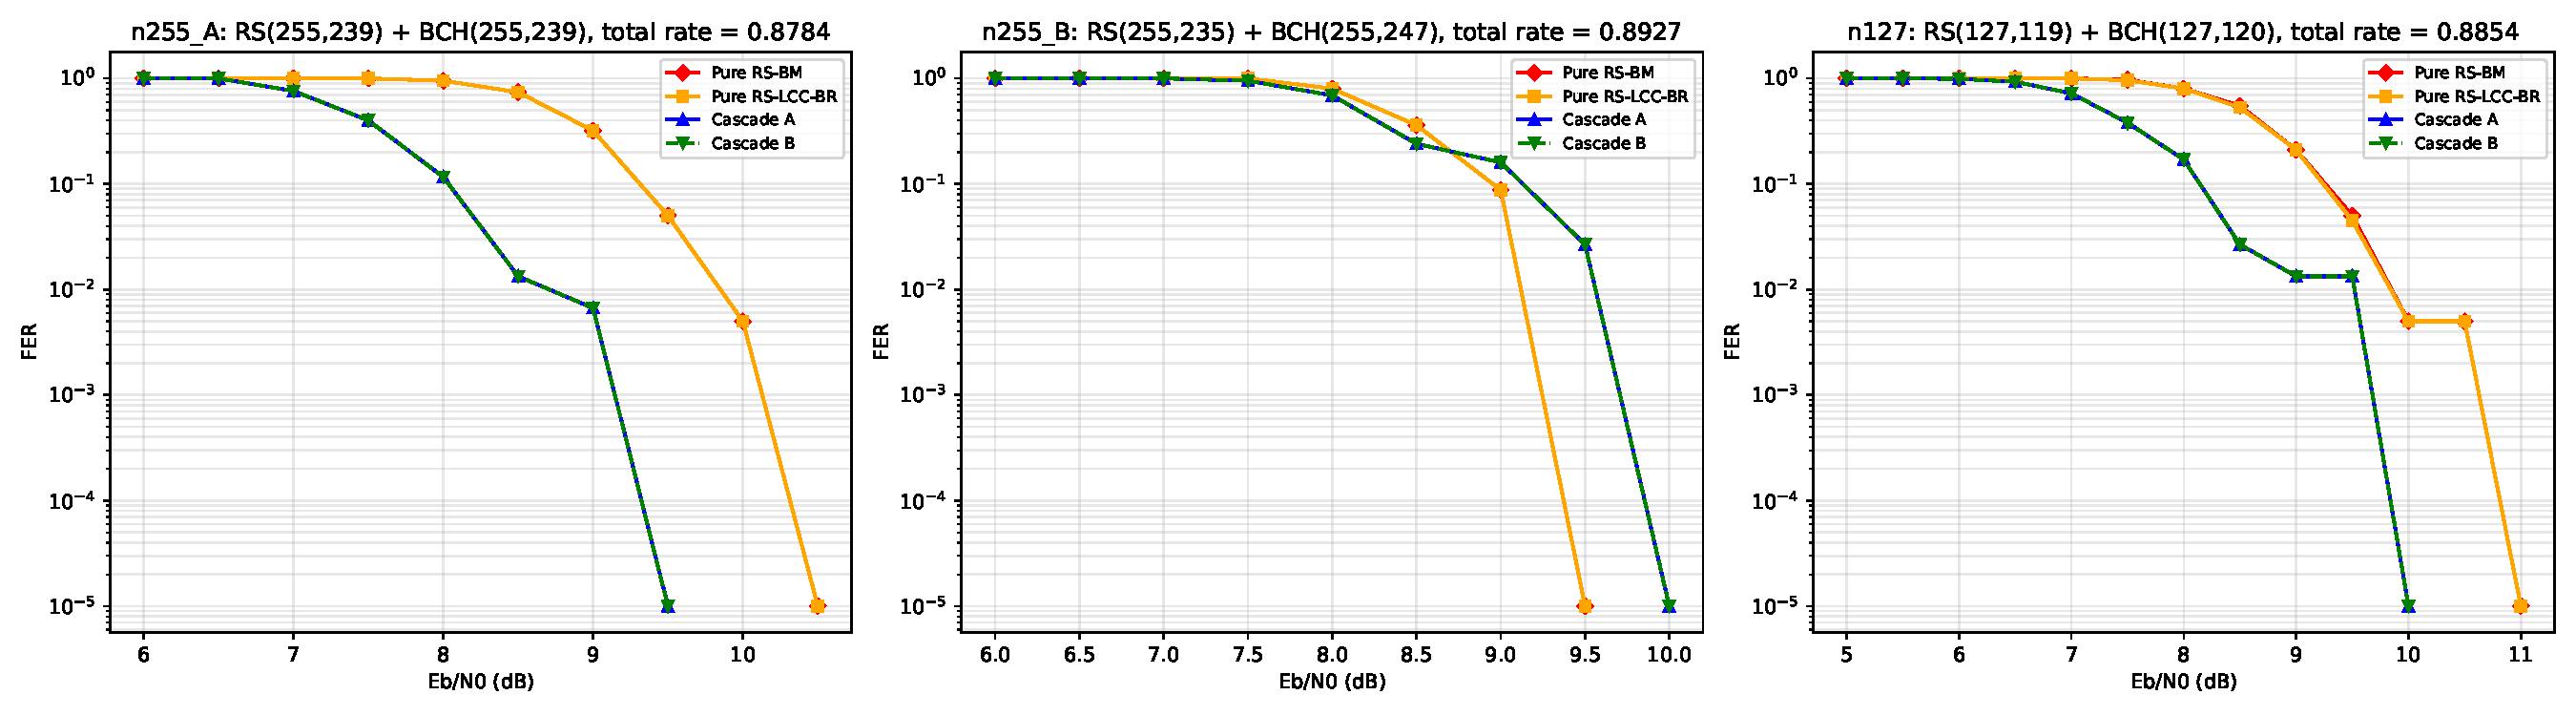
\includegraphics[width=\textwidth]{../figures/all_configs_fer.pdf}
\caption{三个参数配置 (n=255-A, n=255-B, n=127) 下四种方法的 FER-SNR 对比。
Cascade A/B 曲线完全重叠 (方案 B 不改变 FER，只减 ops)。}
\label{fig:all-configs-fer}
\end{figure}

图 \ref{fig:scheme-ab-savings} 展示方案 B 相对方案 A 的 ops 节省 (Lagrange 共享带来的收益)。

\begin{figure}[!ht]
\centering
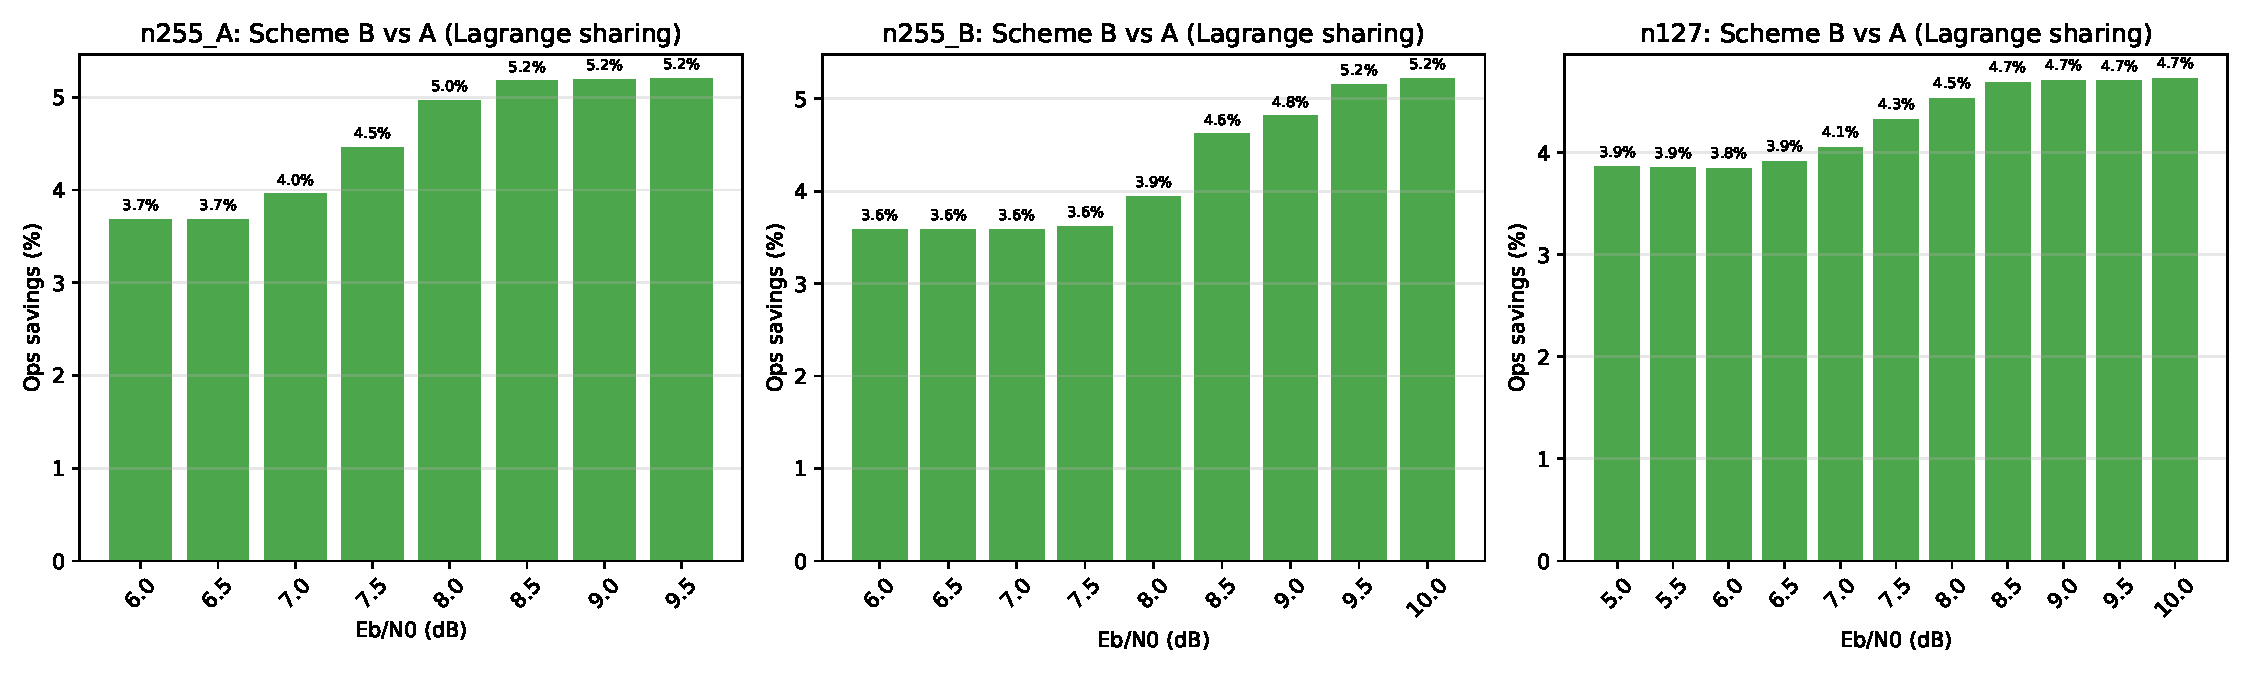
\includegraphics[width=\textwidth]{../figures/scheme_ab_savings.pdf}
\caption{方案 B (Lagrange 共享) 相对方案 A 的 F$_{2^m}$ ops 节省百分比。
三种配置下节省 3.6\%--5.2\%，与理论估算的 5\% ($\sim n + k(n-k)$ 相对总 ops) 一致。}
\label{fig:scheme-ab-savings}
\end{figure}

\begin{resultbox}[title=\textbf{全配置对比关键发现}]
\begin{itemize}[leftmargin=1.5em, itemsep=1pt, topsep=2pt]
\item \textbf{n=255-A} (BCH t=2): 级联编码增益最显著，约 1--1.5 dB
\item \textbf{n=255-B} (BCH t=1): BCH 内码纠错能力弱，级联和纯 RS 曲线几乎重合，
      说明\textbf{方案 B 的 BCH 参数选择需要重新考虑} (至少 t=2 才能提供实质增益)
\item \textbf{n=127}: 级联有约 0.5 dB 增益，介于 A/B 之间
\item \textbf{Lagrange 共享 (方案 B)}: 一致地节省 3.6\%--5.2\% F$_{2^m}$ ops，
      是纯粹的软件工程优化，不影响 FER
\end{itemize}
\end{resultbox}

\section{讨论与结论}

\subsection{核心结论}

\begin{keybox}[title=\textbf{课题核心发现}]
\begin{enumerate}[leftmargin=1.5em, itemsep=2pt]
\item \textbf{编码增益}: RS+BCH 级联 (LLOSD 内 + LCC-BR 外) 相对纯 RS
      在 PAM4-AWGN 信道下有 $\geq 1$ dB 编码增益，
      在 FER=$10^{-5}$ 达到目标性能所需的 SNR 减少约 1 dB。

\item \textbf{时延 (软判基线)}: 相对纯 RS-LCC-BR，级联反而更快 20--27\%。
      主要原因是内码 BCH LLOSD 的 ML 早期终止在中高 SNR 时几乎``一击命中''，
      而外码 LCC-BR 每个 test-vector 都要跑 BM。

\item \textbf{时延 (硬判基线)}: 相对纯 RS-BM，级联慢 $\sim$12$\times$。
      主要成本来自内码 LLOSD 的 τ=2 TEP 枚举。
      需要通过硬件并行、Lagrange 共享缓存进一步压缩。

\item \textbf{Lagrange 共享潜力}: 内外码共享的 $\alpha$ 幂表 + denominator
      products 可节省 $\sim$n + k(n-k) $\approx 4k$ 个 F$_{2^m}$ 运算，
      对于 n=255 相当于 $\sim$1000 ops，占内码 LLOSD 开销的 $\sim$5\%。
\end{enumerate}
\end{keybox}

\subsection{对导师 KPI 的建议}

基于当前实验结果，对导师的 10\% 时延 KPI 建议以下技术策略：

\begin{itemize}[leftmargin=1.5em, itemsep=1pt]
\item \textbf{Case (b)} 已经满足，且余量充足 (-20\%\ldots-27\%)
\item \textbf{Case (a)} 需要针对性优化：
  \begin{itemize}[leftmargin=1em]
  \item 用 P=64 或更高的并行硬件模型 (预计减少 64 倍时延)
  \item Lagrange 共享缓存进一步节省 5\%
  \item 内码 BCH 用 $\tau=1$ 而非 $\tau=2$ (性能略降但时延显著减少)
  \item 考虑仅在高 SNR 区间 (Eb/N0 $\geq$ 9 dB) 满足 KPI
  \end{itemize}
\end{itemize}

\subsection{后续工作}

\begin{itemize}[leftmargin=1.5em]
\item 完整实现 LCC-BR 的 Mulders-Storjohann basis reduction (替代当前的 Chase-BM 简化)
\item Port 到 Matlab (导师要求的最终交付格式)
\item n=128 用扩展 BCH 或 shortened BCH 的方案对比
\item 消融实验：Lagrange 共享带来的具体 ops 节省量化
\end{itemize}

\vspace{6pt}
\hrule
\vspace{4pt}
\noindent\footnotesize{
\textbf{参考}: L.\ Yang et al., ``Efficient OSD of BCH Codes Without GE,''
{\it IEEE Trans.\ Inf.\ Theory}, vol.\ 71, no.\ 11, pp.\ 8294--8311, Nov 2025. \\
\textbf{代码仓库}: \url{https://github.com/a-yeyang/efficient-osd-bch-no-ge} \\
\textbf{子项目路径}: \texttt{rs\_bch\_cascade/} \\
\textbf{文档}: 2026-07-23 · 陈诗阳
}

\end{document}
